% Compiler depuis ce dossier : latexmk -pdf main.tex
\documentclass[11pt,a4paper]{report}
% Préambule du rapport : compilation depuis main.tex.
% Les textes de couverture et les couleurs peuvent être modifiés ci-dessous.
\usepackage[T1]{fontenc}
\usepackage[utf8]{inputenc}
\IfFileExists{french.ldf}{%
  \usepackage[french]{babel}
}{%
  \usepackage{babel}
  \babelprovide[main,import]{french}
}
\usepackage{lmodern}
\usepackage{microtype}
\usepackage[a4paper,left=23mm,right=23mm,top=25mm,bottom=21mm]{geometry}
\usepackage{graphicx}
\usepackage{xcolor}
\usepackage{amsmath,amssymb}
\usepackage{booktabs,tabularx,array,longtable}
\usepackage{ragged2e}
\usepackage{caption}
\usepackage{placeins}
\usepackage{titlesec}
\usepackage{tikz}
\usetikzlibrary{arrows.meta,positioning}
\usepackage{hyperref}
\usepackage{xurl}
\setlength{\parindent}{0pt}
\clubpenalty=10000
\widowpenalty=10000
\displaywidowpenalty=10000

\definecolor{anthracite}{HTML}{252728}
\definecolor{terreCuite}{HTML}{A5553E}
\definecolor{grisTexte}{HTML}{62666A}
\definecolor{grisCredit}{HTML}{7B7E81}
\newcolumntype{L}{>{\raggedright\arraybackslash}X}
\newcommand{\nomChapitre}{CHAPITRE}
\newcommand{\code}[1]{{\ttfamily\small\expandafter\nolinkurl\expandafter{\detokenize{#1}}}}
\newcommand{\sourcecalcul}[1]{\par\vspace{2pt}{\footnotesize\color{grisTexte}Source : #1.\par}}
\newcommand{\bilan}[1]{\par\medskip\noindent{\sffamily\bfseries À retenir. }#1\par}
\captionsetup{font=small,labelfont=bf,skip=7pt,justification=raggedright,singlelinecheck=false}
\renewcommand{\figurename}{Figure}
\renewcommand{\tablename}{Tableau}
\setlength{\textfloatsep}{14pt plus 3pt minus 2pt}
\setlength{\intextsep}{12pt plus 3pt minus 2pt}
\setlength{\floatsep}{12pt plus 3pt minus 2pt}
\renewcommand{\topfraction}{0.90}
\renewcommand{\bottomfraction}{0.80}
\renewcommand{\textfraction}{0.08}
\renewcommand{\floatpagefraction}{0.72}
\setcounter{topnumber}{3}
\setcounter{bottomnumber}{2}
\titleformat{\chapter}[display]
  {\sffamily\bfseries\raggedright\color{anthracite}}
  {\color{terreCuite}\fontsize{11}{14}\selectfont \nomChapitre\ \thechapter}
  {8pt}{\fontsize{24}{29}\selectfont}
  [\vspace{3mm}{\color{terreCuite}\rule{18mm}{1.2pt}}]
\titlespacing*{\chapter}{0pt}{0pt}{17pt}
\titleformat{\section}{\sffamily\large\bfseries\color{anthracite}}{\thesection}{0.7em}{}
\titlespacing*{\section}{0pt}{15pt}{7pt}
\titleformat{\subsection}{\sffamily\normalsize\bfseries\color{anthracite}}{\thesubsection}{0.7em}{}
\titlespacing*{\subsection}{0pt}{10pt}{5pt}
\titleformat{\part}[display]{\centering\sffamily\bfseries\color{anthracite}}
  {\color{terreCuite}\Large PARTIE \thepart}{18pt}{\fontsize{27}{34}\selectfont}

\newcommand{\titreRapport}{Ring-Star :\\concevoir une ligne\\de transport circulaire}
\newcommand{\sousTitreRapport}{Modélisation mathématique, heuristiques\\et comparaison expérimentale}
\newcommand{\perimetreRapport}{Recherche opérationnelle\enspace\(\cdot\)\enspace Huit instances de 16 à 100 points}
\newcommand{\auteurRapport}{Papa Birane Mbengue}
\newcommand{\formationRapport}{Élève ingénieur en informatique - Sup Galilée}
\newcommand{\dateRapport}{Octobre 2026}
\newcommand{\imageCouverture}{figures/couverture_ring_star.png}
\newcommand{\creditPhoto}{Source : researchgate.net ; illustration de Liefooghe, Jourdan et Talbi (2008).}

\hypersetup{
  pdftitle={Ring-Star : concevoir une ligne de transport circulaire},
  pdfauthor={Papa Birane Mbengue},
  pdfsubject={Modélisation mathématique et comparaison des méthodes de résolution du Ring-Star},
  hidelinks
}

\usepackage{fvextra}
\DefineVerbatimEnvironment{commandes}{Verbatim}{fontsize=\small,breaklines=true,breakanywhere=true}
\newcommand{\figureRS}[4][0.98]{%
  \begin{figure}[htbp]\centering
  \includegraphics[width=#1\textwidth]{figures/#2}
  \caption{#3}\label{#4}
  \sourcecalcul{exécutions enregistrées du projet Ring-Star, campagne du 17 octobre 2026.}
  \end{figure}%
}
\newcommand{\sourcetable}{\sourcecalcul{exports JSON et CSV de la campagne de démonstration ; tableaux régénérés sans relancer les solveurs.}}
\newcommand{\exigence}[2]{\textbf{#1.} #2\par}

\newcommand{\titrePreliminaire}[1]{%
  {\sffamily\color{anthracite}\bfseries\fontsize{24}{29}\selectfont #1\par}%
  \vspace{5mm}{\color{terreCuite}\rule{18mm}{1.2pt}\par}\vspace{8mm}}
\renewcommand{\contentsname}{Sommaire}
\setcounter{tocdepth}{1}
\begin{document}
\renewcommand{\figurename}{Figure}
\renewcommand{\tablename}{Tableau}
\begin{titlepage}
\thispagestyle{empty}
\sffamily\color{anthracite}

% Repère de couleur discret et composition alignée à gauche.
{\color{terreCuite}\rule{18mm}{1.6pt}\par}
\vspace{9mm}

{\bfseries\fontsize{30}{36}\selectfont \titreRapport\par}
\vspace{7mm}

{\fontsize{14}{20}\selectfont \sousTitreRapport\par}
\vspace{6mm}

{\color{grisTexte}\fontsize{10.5}{15}\selectfont \perimetreRapport\par}
\vspace{20mm}

% Photographie fournie par l'auteur, conservée dans son cadrage d'origine.
\includegraphics[width=\textwidth]{\imageCouverture}\par
\vspace{2mm}
{\color{grisCredit}\fontsize{8}{11}\selectfont \creditPhoto\par}

\vfill
\begin{minipage}[b]{0.76\textwidth}
  {\bfseries\fontsize{12}{16}\selectfont \auteurRapport\par}
  \vspace{1.5mm}
  {\color{grisTexte}\fontsize{9.5}{13}\selectfont \formationRapport\par}
\end{minipage}\hfill
\begin{minipage}[b]{0.22\textwidth}
  \raggedleft
  {\color{grisTexte}\fontsize{10}{14}\selectfont \dateRapport\par}
\end{minipage}
\end{titlepage}

\pagenumbering{roman}
\pagestyle{plain}
\color{anthracite}
\setlength{\parskip}{7pt}
\setlength{\emergencystretch}{2em}
\fontsize{11}{15}\selectfont
\pdfbookmark[0]{Résumé}{resume}
\titrePreliminaire{Résumé}
Ce projet étudie le choix des stations et le tracé d'une ligne de transport circulaire
au moyen du problème Ring-Star, ou anneau-étoile. Parmi $n$ points candidats,
exactement $p$ deviennent des stations, dont un sommet imposé. Les stations sont
reliées par un cycle unique et chaque autre point est affecté à une station.
Le coût additionne la longueur du cycle, pondérée par $\alpha$, et les distances
d'accès aux stations. Le modèle représente une décision de localisation et de
routage ; il ne constitue pas une étude opérationnelle d'un réseau de transport réel.

Le travail reprend l'énoncé de la SAÉ Optimisation de Sup Galilée et en explicite
les hypothèses. Lorsque $p=n$ et $\alpha>0$, le problème contient le voyageur de
commerce euclidien comme cas particulier, ce qui établit sa NP-difficulté.
La résolution exacte repose sur une programmation linéaire en nombres entiers
avec des variables d'affectation, des arêtes d'anneau et un flot assurant la
connexité. Le modèle est construit avec PuLP et résolu par CBC.

Trois méthodes approchées complètent cette formulation. Une construction
déterministe choisit les stations à partir d'une grille, affecte les points à leur
station la plus proche et construit un cycle par plus proche voisin, amélioré
par 2-opt. Une recherche locale accepte les échanges de stations améliorants.
Une recherche tabou peut accepter une dégradation temporaire, interdit certains
retours et conserve la meilleure solution rencontrée.

L'évaluation principale porte sur huit nuages de points issus de TSPLIB, de 16 à
100 sommets, avec $p\in\{3,5,10\}$ et $\alpha=1$. Les deux recherches sont répétées
sur trois graines. Le protocole compte 192 cas de méthode et de graine :
168 exécutions heuristiques, quatre résolutions PLNE et 20 cas PLNE ignorés
par les limites de taille configurées. Sur les quatre PLNE exécutés, trois
aboutissent à une preuve d'optimalité et un fournit une solution réalisable
sans preuve dans le budget de cinq secondes.

Les gains médians de coût face à la construction sont de 11,79\,\% pour la
recherche locale et de 13,67\,\% pour la recherche tabou, en donnant le même poids
à chacun des 24 cas d'instance et de cardinalité. La moyenne tabou est inférieure
à la moyenne locale dans 22 cas et égale dans deux cas. Ce constat est lié au
protocole : une itération tabou évalue jusqu'à 15 échanges, contre un seul pour
la recherche locale. Il ne démontre donc pas une supériorité à effort de calcul égal.

L'étude détaillée d'\code{att48}, avec dix stations, illustre une baisse du coût
de 48\,833,89 à 42\,743,75, soit 12,47\,\%. La reproductibilité repose sur la
conservation des coordonnées, des paramètres, des solutions, des traces et des
versions logicielles. Les 172 solutions de la campagne ont été relues et leurs
coûts recalculés pour le rapport. La suite de 101 tests passe également avec
un contrôle renforcé de l'export des cas ignorés.

\vspace{3mm}
{\sffamily\small\raggedright\textbf{Mots-clés :} recherche opérationnelle, Ring-Star,
localisation-routage, PLNE, recherche tabou, expérimentation reproductible.\par}

\clearpage
\pdfbookmark[0]{Sommaire}{sommaire}
\renewcommand{\contentsname}{Sommaire}
{\setlength{\parskip}{0pt}\fontsize{10}{12.5}\selectfont\tableofcontents}
\clearpage
\pagenumbering{arabic}
\phantomsection
\titrePreliminaire{Introduction générale}
\addcontentsline{toc}{chapter}{Introduction générale}
Concevoir une ligne de transport circulaire demande de choisir les lieux desservis
et l'ordre dans lequel les relier. Desservir davantage de zones peut raccourcir
l'accès des usagers, mais allonge parfois la ligne. À l'inverse, concentrer les
stations peut produire un anneau court tout en éloignant certains points de leur
station d'accès. Les deux décisions ne peuvent donc pas être traitées comme des
objectifs entièrement indépendants.

Le problème Ring-Star représente cette interaction dans un cadre géométrique
simple. Un anneau relie une partie des points ; les autres lui sont rattachés par
des arcs d'affectation. Le schéma de couverture illustre cette structure, avec les
arêtes du cycle en trait plein et les affectations en pointillé. Il est emprunté à
une publication consacrée à une variante bi-objective du problème\cite{figure}.
Le présent projet retient une somme pondérée des deux coûts et fixe le nombre
de stations, conformément à l'énoncé de la SAÉ\cite{enonce}.

La problématique étudiée est la suivante :
\begin{quote}\itshape
Comment sélectionner un nombre fixé de stations et construire leur cycle pour
réduire conjointement la longueur de la ligne et les distances d'accès, et quel
compromis entre qualité, temps de calcul et garantie offrent les méthodes proposées ?
\end{quote}

Une solution exacte sert de référence lorsque le problème et le budget de calcul
le permettent. Des méthodes approchées produisent rapidement des solutions
réalisables et cherchent à améliorer leur coût. La comparaison doit prendre en
compte la variabilité des recherches, le travail effectivement réalisé et le
statut des résultats du solveur. Une valeur renvoyée par une formulation exacte
ne devient pas un optimum prouvé du seul fait de l'utilisation d'une PLNE.

Ce rapport présente les méthodes effectivement implémentées dans le projet et
les résultats enregistrés de sa campagne de démonstration. Il explique les choix
de représentation, les règles de calcul et les contrôles qui permettent de relier
une figure à une solution précise. Les tableaux sont calculés depuis les exports
archivés ; aucune nouvelle campagne de grande ampleur n'est supposée réalisée.

La première partie développe le cadrage, la formulation mathématique, la
NP-difficulté, la PLNE et les trois méthodes approchées. La seconde décrit le
protocole, interprète les résultats, approfondit un cas sur \code{att48} et examine
la qualité logicielle ainsi que les limites de l'étude. Un glossaire et des annexes
permettent de retrouver les notations, les commandes et l'ensemble des coûts.

\clearpage
\part{Modélisation et méthodes de résolution}
\chapter{Cadrage du projet et cahier des charges}
\section{Finalité et périmètre}
Le projet s'inscrit dans la SAÉ « Autour du tracé d'un métro circulaire » de
Sup Galilée\cite{enonce}. Le sujet demande notamment de justifier la NP-difficulté,
de visualiser les données et les solutions, de programmer une heuristique et une
métaheuristique, d'implémenter une formulation compacte et de comparer les méthodes.
La version étudiée fournit en plus une recherche locale distincte de la recherche
tabou, des campagnes à plusieurs graines et des résultats consultables par des
résumés Markdown.

Un point représente une zone candidate à l'implantation d'une station. Les points
ont tous le même poids dans le coût d'accès : aucune population, demande ou
fréquence de déplacement n'est fournie. Les distances sont calculées à vol
d'oiseau dans le plan des coordonnées. Elles ne décrivent ni un chemin dans la
voirie ni une durée de transport. Le mot « coût » désigne ici la fonction objectif,
sans conversion en euros.

\section{Entrées et décisions attendues}
Les entrées sont un fichier de coordonnées, un nombre de stations $p$, un poids
$\alpha$ et les paramètres de la méthode. Le premier sommet du fichier est une
station imposée. Les bornes retenues sont $3\leq p\leq n$ et $0\leq\alpha\leq10$.
Le code utilise des indices internes de 0 à $n-1$ ; les exports lisibles numérotent
les points de 1 à $n$. Ainsi, le sommet imposé habituel est 0 en interne et 1
dans les résultats.

Une sortie complète contient l'ensemble des stations, l'ordre du cycle, une
affectation par point et les trois coûts : anneau non pondéré, accès et total
pondéré. Elle précise aussi la méthode, la graine, les budgets et le statut.
Pour les recherches, les traces distinguent le coût courant de la meilleure
valeur rencontrée. Pour CBC, la preuve d'optimalité et la borne inférieure sont
des informations séparées de la solution réalisable.

\section{Exigences de qualité}
\exigence{Réalisabilité}{Toute solution doit comporter exactement $p$ stations,
inclure le sommet imposé et former un cycle simple passant par chacune d'elles.
Chaque point est affecté à une station ouverte et chaque station à elle-même.}
\exigence{Cohérence numérique}{Les méthodes partagent la même matrice de distances
et la même évaluation du coût. Les coordonnées non finies et les paramètres
hors domaine sont rejetés avant l'optimisation.}
\exigence{Comparabilité}{Les méthodes approchées partent de la même construction
pour un cas fixé. Les comparaisons conservent l'instance, $p$ et $\alpha$ ; les
statistiques ne mélangent pas des problèmes différents.}
\exigence{Traçabilité}{Une figure est reliée à une solution sauvegardée. Les
coordonnées et l'ordre du cycle sont conservés pour régénérer la figure sans
recalculer un autre parcours.}
\exigence{Utilisation}{L'installation, les tests et les exécutions sont accessibles
par une interface de commande et un Makefile. Les résultats individuels et les
campagnes possèdent chacun un point d'entrée documenté.}

\section{État du travail étudié}
Le dépôt public est \href{https://github.com/birane-m/ring-star-problem}{birane-m/ring-star-problem}.
Les trois commits publiés jusqu'à \code{8761003} regroupent le code expérimental,
les outils du projet et la documentation. Les calculs présentés ont été enregistrés
le 17 octobre 2026 ; leur empreinte de sources est conservée dans les métadonnées.
Ils précèdent les dernières modifications de présentation et ne sont pas
présentés comme une campagne relancée après chaque commit.

Le contrôle documentaire a identifié une écriture finale manquante du CSV pour
un cas PLNE ignoré. La correction jointe aux sources ne modifie aucun algorithme
ni aucun coût ; elle fiabilise la complétude de l'export. Son statut et les
contrôles associés sont explicités au chapitre~\ref{chap:qualite}.
\bilan{Le projet répond à une question de localisation-routage dans un modèle
géométrique défini. La validité des comparaisons dépend autant des conventions
communes et des budgets que des valeurs finales des coûts.}

\chapter{Modèle mathématique et difficulté du problème}
\section{Une solution sous forme d'anneau et d'affectations}
Soit $V=\{1,\ldots,n\}$ l'ensemble des points et $r\in V$ le sommet imposé.
Pour des coordonnées $(x_i,y_i)$, le projet définit
\begin{equation}
d_{ij}=\sqrt{(x_i-x_j)^2+(y_i-y_j)^2}.
\end{equation}
Ces distances sont symétriques, positives ou nulles, et non arrondies. Le graphe
est complet : une arête peut relier n'importe quelle paire de points.

Une solution est un triplet $(S,\pi,a)$. L'ensemble $S\subseteq V$ contient les
$p$ stations et vérifie $r\in S$. Le vecteur $\pi=(\pi_1,\ldots,\pi_p)$ est une
permutation de $S$, qui définit les arêtes du cycle en posant $\pi_{p+1}=\pi_1$.
L'affectation $a(i)\in S$ associe chaque point à une station, avec $a(i)=i$
pour les stations.

Le cycle est \emph{simple au sens combinatoire} : aucune station n'est répétée
dans la permutation. Cette propriété n'interdit pas, à elle seule, un croisement
géométrique de deux segments. Le recours à 2-opt améliore le parcours euclidien,
sans ajouter explicitement une contrainte géométrique d'absence de croisement.

\section{Fonction objectif et affectation optimale à stations fixées}
Les deux composantes sont
\begin{equation}
L(S,\pi)=\sum_{k=1}^{p}d_{\pi_k,\pi_{k+1}},\qquad
A(S,a)=\sum_{i\in V}d_{i,a(i)}.
\end{equation}
Le problème minimise
\begin{equation}\label{eq:objectif}
C(S,\pi,a)=\alpha L(S,\pi)+A(S,a).
\end{equation}
Les stations contribuent zéro à $A$, puisqu'elles s'affectent à elles-mêmes.
La longueur $L$ est comptée une seule fois sur le cycle fermé. Il ne s'agit pas
de la somme des trajets en transport de tous les voyageurs : aucun couple
origine-destination n'est modélisé.

Lorsque $S$ est fixé, les affectations sont indépendantes les unes des autres.
Il n'existe ni capacité de station ni quota d'usagers. On peut donc choisir
\begin{equation}
a(i)\in\mathop{\mathrm{arg\,min}}_{s\in S}d_{is},\qquad
A(S)=\sum_{i\in V}\min_{s\in S}d_{is}.
\end{equation}
Toute affectation plus lointaine peut être remplacée par une plus proche sans
modifier l'anneau et sans augmenter le coût. Les heuristiques exploitent cette
propriété à chaque échange de stations. En cas d'égalité de distance, elles
choisissent le plus petit indice pour rendre la décision déterministe.

\section{Deux problèmes classiques intégrés}
La sélection des stations rappelle le problème du $p$-médian, qui minimise la
somme des distances d'accès. Une fois les stations fixées, la recherche du
meilleur ordre de visite est un problème du voyageur de commerce sur $S$.
L'intégration vient du fait que choisir $S$ en ne regardant que les accès peut
produire un anneau coûteux. La meilleure sélection dépend donc de $\alpha$.

Pour $\alpha=0$, seul le coût d'accès intervient. Le problème devient un
$p$-médian avec un centre imposé ; le cycle reste requis pour la représentation,
mais son ordre n'influe plus sur l'objectif. Pour $p=n$, toutes les affectations
ont un coût nul. Si $\alpha>0$, il ne reste que le choix du cycle.

Une augmentation de $\alpha$ renchérit toute solution fixée dont l'anneau est
non nul, mais peut aussi conduire à sélectionner d'autres stations. De même,
augmenter $p$ ne garantit pas une diminution du coût total : une meilleure
couverture et une ligne plus longue peuvent se compenser. Les graphiques selon
$p$ doivent ainsi être lus comme des compromis, et non comme une courbe de
performance qui devrait forcément décroître.

\section{Justification de la NP-difficulté}
Considérons une instance du voyageur de commerce euclidien symétrique à $n$
points, avec $n\geq3$. Construisons une instance Ring-Star ayant les mêmes points,
les mêmes distances, $p=n$, $\alpha=1$ et un sommet imposé quelconque.
Cette transformation demande un temps polynomial.

Comme exactement $n$ stations sont requises, tous les points sont sélectionnés.
Le coût des affectations est nul et le coût Ring-Star est exactement la longueur
du cycle hamiltonien. Le sommet imposé ne retire aucune solution, puisque tout
cycle hamiltonien visite tous les sommets. Une résolution optimale du Ring-Star
donnerait donc une résolution optimale du voyageur de commerce euclidien.
Ce dernier étant NP-difficile, le problème Ring-Star général l'est également.

Cette réduction porte sur un cas particulier autorisé, avec $\alpha=1$.
Elle ne dit pas que chaque instance est difficile ni que le cas dégénéré
$\alpha=0$, $p=n$ l'est. Elle justifie le recours aux heuristiques et la nécessité
de limiter certaines résolutions exactes. Il suffit ici d'établir la
NP-difficulté ; aucune affirmation supplémentaire sur l'appartenance à NP avec
des distances euclidiennes exactes n'est nécessaire.
\bilan{Le coût combine deux décisions liées. Les affectations sont simples à
optimiser lorsque les stations sont fixées, mais la sélection des stations et
l'ordre de leur cycle rendent le problème combinatoire.}

\chapter{Résolution exacte par une formulation compacte}
\section{Variables et objectif}
La formulation utilise le graphe non orienté complet $G=(V,E)$ et les arcs
orientés $D=\{(i,j):i\ne j\}$ associés aux arêtes. Elle s'appuie sur quatre
familles de variables :
\begin{itemize}
\item $z_i\in\{0,1\}$ indique si $i$ est une station ;
\item $y_{ij}\in\{0,1\}$ indique si le point $i$ est affecté à la station $j$ ;
\item $x_{ij}\in\{0,1\}$, pour $\{i,j\}\in E$, indique si cette arête appartient à l'anneau ;
\item $f_{ij}\geq0$, pour $(i,j)\in D$, désigne un flot fictif de connexité.
\end{itemize}
Le flot n'est pas un flux de voyageurs. C'est un outil mathématique qui empêche
la formation de plusieurs cycles disjoints. L'objectif est
\begin{equation}
\min\;\alpha\sum_{\{i,j\}\in E}d_{ij}x_{ij}
       +\sum_{i\in V}\sum_{j\in V}d_{ij}y_{ij}.
\end{equation}

\section{Sélection, affectation et degré}
Le nombre de stations et la présence du sommet imposé s'écrivent
\begin{equation}
\sum_{i\in V}z_i=p,\qquad z_r=1.
\end{equation}
Les affectations vérifient
\begin{align}
\sum_{j\in V}y_{ij}&=1 &&\forall i\in V,\\
y_{ij}&\leq z_j &&\forall i,j\in V,\\
y_{ii}&=z_i &&\forall i\in V.
\end{align}
Ces égalités imposent une affectation unique, exclusivement vers une station
ouverte, ainsi que l'auto-affectation des stations. L'objectif choisit une station
la plus proche à l'optimum, sans avoir à coder cette règle sous forme de
contraintes supplémentaires.

Chaque station possède deux arêtes d'anneau ; un point non retenu n'en possède
aucune :
\begin{equation}
\sum_{j\in V\setminus\{i\}}x_{\{i,j\}}=2z_i\qquad\forall i\in V.
\end{equation}
Le programme ajoute également les liaisons $x_{ij}\leq z_i$ et $x_{ij}\leq z_j$.
Dans une solution binaire, le degré exclut déjà les arêtes incidentes aux
non-stations, mais ces liaisons rendent cette relation explicite dans le modèle.

\section{Éliminer les cycles disjoints par un flot}
Les seules contraintes de degré permettraient plusieurs cycles séparés. Pour
obtenir un cycle unique, la racine émet $p-1$ unités de flot et chaque autre
station en consomme une :
\begin{align}
\sum_{j\ne r}f_{rj}-\sum_{j\ne r}f_{jr}&=p-1,\\
\sum_{j\ne i}f_{ji}-\sum_{j\ne i}f_{ij}&=z_i
   &&\forall i\ne r.
\end{align}
Le flot ne peut emprunter qu'une arête retenue :
\begin{equation}
f_{ij}+f_{ji}\leq(p-1)x_{ij}\qquad\forall\{i,j\}\in E.
\end{equation}
Les variables sont aussi bornées individuellement par $p-1$ dans le code.

Pour comprendre la connexité, supposons qu'un ensemble non vide de stations
forme une composante qui ne contient pas $r$. En additionnant ses équations de
conservation, les flots internes se compensent et la demande totale reste
strictement positive. Or aucune arête active ne relie cette composante au reste
du graphe, donc aucun flot ne peut y entrer. C'est une contradiction.
Le graphe actif est ainsi connexe. Comme ses sommets ont tous degré deux et
$p\geq3$, il forme un unique cycle.

Réciproquement, tout cycle réalisable admet un flot de $p-1,p-2,\ldots,1$
unités le long d'un sens du cycle, chaque station consommant une unité.

\section{Taille du modèle et outil de résolution}
Le modèle contient $n$ variables de station, $n^2$ d'affectation,
$n(n-1)/2$ d'arête et $n(n-1)$ de flot. Ses nombres de variables et de contraintes
sont d'ordre $n^2$ : c'est une formulation \emph{compacte}, ce qui ne rend pas
sa résolution entière polynomiale.

PuLP construit le modèle et appelle CBC, solveur de programmation entière
à séparation et évaluation arborescente\cite{cbc}. Le projet conserve le journal,
reconstruit le cycle et valide la solution. Il ne programme pas de séparation
de sous-tours ni d'arbre de Gomory-Hu ; la formulation non compacte reste
une extension possible.

\section{Une méthode exacte peut s'arrêter sans preuve}
Le programme contrôle les statuts du modèle et de la solution, vérifie
l'intégralité des décisions binaires puis recalcule le coût. Il annonce
\code{optimal} uniquement avec une preuve. Sous budget, une solution entière
sans preuve est classée \code{feasible_time_limited}. Sans solution utilisable,
aucun coût n'est inventé.

Si le journal fournit une borne inférieure $B$ compatible avec le coût
réalisable $C$, l'export conserve $g_B=(C-B)/\max(|C|,10^{-12})$.
Une borne absente reste absente. Cet écart se distingue de celui à un
optimum prouvé, défini au chapitre~\ref{chap:protocole}.

\chapter{Construire une première solution réalisable}
\section{Pourquoi commencer par une référence simple}
Une construction rapide fournit à la fois une solution immédiatement utilisable
et un point de départ commun aux recherches. Elle aide à mesurer ce que
l'amélioration apporte réellement. Le terme \code{greedy} de l'interface désigne
ici une chaîne de règles déterministes : sélection géométrique par grille,
affectation au plus proche, construction du cycle puis amélioration 2-opt.
Ce n'est pas une optimisation exacte de chacun de ces sous-problèmes.

La matrice des distances est calculée une seule fois par exécution et partagée
par les étapes suivantes. Tous les coûts utilisent les distances non arrondies.
Les règles d'égalité sur les indices rendent la construction reproductible sans
avoir à répéter artificiellement la même méthode sur plusieurs graines.

\section{Choisir les stations avec une grille}
On calcule le rectangle englobant le nuage de points, puis
$q=\lceil\sqrt{p}\rceil$. Le rectangle est partagé en $q\times q$ cellules.
Dans chaque cellule non vide, on choisit le point le plus proche du centre de
la cellule. La frontière supérieure de la dernière ligne et de la dernière
colonne est incluse pour ne pas perdre les points extrêmes.

Cette règle couvre spatialement le nuage, mais ne fournit pas nécessairement
$p$ stations : des cellules sont vides, $q^2$ peut dépasser $p$ et l'ajout de
la station imposée modifie le compte. Le programme ajuste donc la sélection.
S'il manque des stations, il ajoute le point dont la distance à la station déjà
sélectionnée la plus proche est maximale. Cette complétion privilégie les zones
encore éloignées d'une station. Si la sélection est trop grande, il retire des
stations jugées redondantes par leur proximité aux autres, en préservant la
station imposée.

Le critère de complétion n'est pas une minimisation exacte de la somme des
accès : c'est une règle de couverture. De même, la grille ignore le coût futur
de l'anneau et le poids $\alpha$. Cette simplification explique pourquoi une
recherche sur les stations peut ensuite réduire sensiblement le coût global.

\section{Affecter les points et ordonner les stations}
Une fois $S$ fixé, chaque point non-station est affecté à la station la plus
proche. Cette étape optimise exactement les affectations conditionnellement à
$S$. Les stations s'affectent à elles-mêmes, même si deux points distincts ont
des coordonnées identiques.

Le cycle démarre au sommet imposé. À chaque étape, la station non visitée la
plus proche de la station courante est ajoutée à la séquence. La dernière
station est ensuite reliée implicitement à la première. La règle du plus proche
voisin évite une énumération de tous les ordres possibles, mais elle peut
conserver des détours liés aux choix effectués plus tôt.

\section{Améliorer le cycle avec 2-opt}
Le mouvement 2-opt enlève deux arêtes $(a,b)$ et $(c,d)$, puis les remplace
par $(a,c)$ et $(b,d)$ en inversant l'ordre du segment intermédiaire.
Pour des distances symétriques, la variation de longueur est
\begin{equation}
\Delta L=d_{ac}+d_{bd}-d_{ab}-d_{cd}.
\end{equation}
Il suffit donc de comparer quatre distances, sans réévaluer tout le cycle
pour chaque paire. L'inversion est retenue si elle raccourcit strictement
le parcours au-delà d'une petite tolérance relative. La recherche reprend
alors sur le nouveau cycle jusqu'à ne plus trouver d'amélioration 2-opt.

La première station reste fixe dans la représentation. Les échanges impliquant
l'arête de fermeture sont autorisés : ignorer cette arête laisserait de côté
des améliorations valides. Un test de non-régression sur un carré vérifie
notamment ce cas.

À stations fixées et pour $\alpha>0$, raccourcir l'anneau réduit le coût total
sans toucher aux affectations. Pour $\alpha=0$, 2-opt améliore seulement la
présentation du cycle ; la valeur de l'objectif est inchangée. La fin de 2-opt
fournit une stabilité vis-à-vis de ce voisinage sur l'ordre des stations, avec
les tolérances numériques du programme. Elle ne prouve pas que le cycle est
un optimum du voyageur de commerce.

\section{Algorithme de construction et coût de calcul}
La procédure peut être résumée sans détailler le code :
\begin{enumerate}
\item Calculer les distances et sélectionner les candidats de la grille.
\item Ajouter la station imposée et ajuster l'ensemble pour obtenir $|S|=p$.
\item Calculer les affectations les plus proches.
\item Construire un cycle par plus proche voisin depuis la racine.
\item Appliquer 2-opt au cycle et vérifier la solution complète.
\end{enumerate}
La matrice demande un temps et une mémoire d'ordre $n^2$. Une affectation
directe demande $O(np)$ comparaisons et le plus proche voisin $O(p^2)$.
Une passe de candidats 2-opt examine $O(p^2)$ échanges ; le nombre de passes
dépend des améliorations réalisées. La version de la grille parcourt les
points pour chaque cellule. Ces choix restent simples à contrôler et adaptés
aux tailles étudiées, sans constituer une démonstration de passage à très
grande échelle.
\bilan{La construction donne une référence déterministe, réalise exactement
les affectations à stations fixées et améliore approximativement l'ordre du
cycle. La sélection reste le principal levier des recherches suivantes.}

\chapter{Améliorer la sélection par recherche locale et tabou}
\section{Un voisinage commun d'échange de stations}
À partir d'un ensemble $S$, on retire une station $u\in S\setminus\{r\}$ et
on ajoute un point $v\in V\setminus S$. Le voisin est défini par
\begin{equation}
S'=(S\setminus\{u\})\cup\{v\}.
\end{equation}
La cardinalité et la présence de la racine sont conservées par construction.
Le nombre de couples possibles vaut $(p-1)(n-p)$. Si $p=n$, aucun échange
n'existe et la recherche s'arrête avec un voisinage vide.

Pour chaque ensemble candidat, les affectations sont recalculées au plus proche,
le cycle est reconstruit par plus proche voisin puis amélioré par 2-opt.
L'évaluation porte sur le coût global $\alpha L+A$, et non sur le seul coût
d'accès. Cette reconstruction permet d'adapter le cycle à la nouvelle sélection,
mais son résultat reste heuristique. Elle ne calcule pas le meilleur cycle
possible pour chaque ensemble candidat.

\section{Recherche locale par échantillonnage}
La recherche locale part de la construction. À chaque itération, elle tire une
station retirable et un point à ajouter, évalue cet unique voisin, puis
l'accepte seulement s'il améliore strictement le coût courant. Un voisin rejeté
laisse la solution inchangée. La meilleure solution est donc aussi la solution
courante et son coût ne croît pas.

L'arrêt intervient lorsque le budget d'itérations ou de temps est atteint,
ou lorsque le voisinage est vide. Comme les voisins sont tirés au hasard et
peuvent être répétés d'une itération à l'autre, l'absence d'amélioration sur
les tirages observés ne prouve pas l'absence d'un meilleur voisin dans
l'ensemble complet. On parle ici de descente échantillonnée, et non de
recherche exhaustive jusqu'à certification d'un optimum local.

La graine initialise un générateur pseudo-aléatoire propre à la recherche.
Les listes de candidats sont triées avant le tirage pour stabiliser les choix.
Cette précaution évite de faire dépendre un résultat de l'ordre d'itération
d'un ensemble Python.

\section{Recherche tabou : accepter des détours contrôlés}
La recherche tabou distingue la solution courante de la meilleure solution
rencontrée. À chaque itération, elle échantillonne sans remise jusqu'à $k$
couples d'échange distincts dans le voisinage courant. Tous les candidats
évalués contribuent au compteur de travail, y compris ceux qui sont ensuite
écartés par la règle tabou.

Le mouvement admissible de plus faible coût est choisi dans cet échantillon.
Il peut dégrader le coût courant. Cette possibilité permet de quitter une
région où une descente stricte resterait bloquée. En parallèle, la meilleure
solution globale n'est remplacée que par une amélioration stricte : le résultat
retourné ne se dégrade donc pas avec les détours de la trajectoire.

Lorsqu'une station est retirée, sa réintroduction est interdite pendant la
durée tabou configurée. Une durée de un bloque bien son retour à l'itération
suivante. L'interdiction porte sur l'ajout du sommet retiré ; elle ne décrit pas
une mémoire de toutes les solutions visitées. Une règle d'aspiration autorise
un mouvement tabou s'il améliore la meilleure valeur globale.

S'il n'existe aucun mouvement admissible dans l'échantillon, la solution
courante reste inchangée et l'itération est comptée. Cela ne signifie pas que
tout le voisinage est interdit. Une nouvelle itération peut échantillonner
d'autres échanges ou bénéficier de l'expiration d'une interdiction.

\section{Déroulé de la recherche tabou}
\begin{enumerate}
\setlength{\itemsep}{1pt}\setlength{\parskip}{0pt}\setlength{\parsep}{0pt}
\item Initialiser la solution courante et la meilleure solution avec la construction.
\item Tirer jusqu'à $k$ échanges distincts et reconstruire leur solution complète.
\item Écarter les mouvements tabous, sauf en cas d'aspiration.
\item Adopter le meilleur mouvement admissible, même s'il dégrade la solution courante.
\item Mettre à jour les interdictions, la meilleure solution et les compteurs.
\item Répéter tant qu'un budget et un voisinage exploitable restent disponibles.
\end{enumerate}
Le nombre de mouvements effectués peut être inférieur au nombre d'itérations.
Ces deux nombres sont exportés séparément, de même que le nombre de candidats
évalués. Le budget est une limite demandée ; les compteurs décrivent le travail
effectivement réalisé.

\section{Budgets et limites de comparaison}
Dans la campagne principale, les deux méthodes disposent de 100 itérations.
La recherche locale évalue donc 100 voisins par exécution. La recherche tabou
évalue 15 voisins à chaque itération, soit 1\,500 dans les cas de cette campagne.
Les voisinages y sont assez grands pour fournir ces 15 couples distincts.
La comparaison porte ainsi sur deux réglages pratiques, avec des efforts différents.

Le budget temporel optionnel des recherches commence après la construction
initiale. Une évaluation déjà commencée peut dépasser légèrement la limite.
Les temps exportés pour l'exécution complète incluent, eux, les distances,
la construction et l'amélioration. Les horloges des traces sont relatives
à la phase d'amélioration ; elles n'ont donc pas exactement la même origine.

Des comparaisons à mêmes nombres d'évaluations et mêmes budgets de temps
permettraient de mieux isoler l'effet du tabou. La campagne temporelle
configurée dans le projet n'a pas été exécutée intégralement.
\bilan{Les deux recherches explorent la même famille d'échanges. La locale
privilégie les améliorations immédiates ; la tabou explore davantage et peut
franchir des dégradations temporaires. Les budgets expliquent une partie
du compromis observé entre coût final et temps.}

\clearpage
\part{Expérimentation, résultats et reproductibilité}
\chapter{Données, protocole et indicateurs}\label{chap:protocole}
\section{Huit nuages de points issus de TSPLIB}
Les fichiers d'entrée proviennent de TSPLIB, bibliothèque de référence pour
le voyageur de commerce\cite{tsplib}. Le projet utilise uniquement les coordonnées
des huit fichiers présents dans le dépôt. Le tableau~\ref{tab:instances} résume
leurs dimensions et leurs types de distance déclarés dans les fichiers sources.
\begin{table}[htbp]\centering
\begin{tabular}{lrrl}
\toprule
Instance & $n$ & $p$ étudiés & Type source \\
\midrule
ulysses16 & 16 & 3, 5, 10 & \code{GEO} \\
ulysses22 & 22 & 3, 5, 10 & \code{GEO} \\
att48 & 48 & 3, 5, 10 & \code{ATT} \\
eil51 & 51 & 3, 5, 10 & \code{EUC_2D} \\
berlin52 & 52 & 3, 5, 10 & \code{EUC_2D} \\
st70 & 70 & 3, 5, 10 & \code{EUC_2D} \\
kroA100 & 100 & 3, 5, 10 & \code{EUC_2D} \\
rd100 & 100 & 3, 5, 10 & \code{EUC_2D} \\
\bottomrule
\end{tabular}

\caption{Instances de la campagne principale. Le type source est conservé comme métadonnée.}
\label{tab:instances}
\sourcecalcul{en-têtes des huit fichiers TSPLIB fournis avec le projet.}
\end{table}

\textbf{La convention de calcul du projet diffère de la métrique officielle
de plusieurs instances.} Toutes les coordonnées sont traitées comme des points
du plan, avec la distance euclidienne non arrondie. La transformation propre
à \code{ATT}, la distance géographique de \code{GEO} et l'arrondi de
\code{EUC_2D} ne sont pas appliqués. Cette convention suit le cadre simplifié
de l'énoncé et rend les méthodes comparables entre elles.

En particulier, les coordonnées des instances Ulysses ne donnent pas ici des
distances physiques en kilomètres. Les optima TSP officiels de TSPLIB ne sont
pas des références valides pour les coûts calculés dans ce projet. Les coûts
bruts de deux instances différentes ne doivent pas non plus être additionnés
ou classés comme s'ils étaient exprimés dans une unité commune.

\section{Plan expérimental réellement exécuté}
Pour chaque instance, trois cardinalités sont retenues : $p=3,5,10$.
Le poids reste fixé à $\alpha=1$, d'où $8\times3=24$ problèmes distincts.
La construction est exécutée une fois. Les recherches locale et tabou sont
répétées sur les graines $0,1,2$, avec 100 itérations chacune. La recherche
tabou utilise une durée de 10 itérations et 15 candidats par itération.

La PLNE n'est tentée que si $n\leq22$ et $p\leq5$, sous une limite de cinq
secondes pour CBC. Elle est exécutée une seule fois dans les cas admissibles,
avec le réglage de solveur enregistré. Les cas qui dépassent les seuils sont
explicitement classés \code{skipped}. Ils ne constituent ni des échecs de
résolution ni des solutions de coût nul.

Au total, le plan contient
\begin{equation}
24\times(1+3+3+1)=192
\end{equation}
enregistrements attendus, en comptant les 20 cas exacts ignorés. Il comporte
172 exécutions avec une solution sauvegardée : 24 constructions, 72 recherches
locales, 72 recherches tabou et quatre PLNE. Parmi ces dernières, trois ont
une preuve et une reste réalisable sans preuve.

Les configurations \code{benchmark_full.json} et
\code{benchmark_time_budget.json} sont proposées pour prolonger l'étude.
La première explore notamment d'autres valeurs de $\alpha$ et davantage de
graines ; la seconde fixe un budget d'amélioration commun. Leur présence
dans le dépôt ne vaut pas résultat expérimental. Le rapport n'attribue donc
aucun effet mesuré au changement de $\alpha$.

\section{Coûts moyens, dispersion et amélioration}
Pour une méthode stochastique et un cas fixé, soient $C_1,\ldots,C_m$ les
coûts des $m$ exécutions réussies. La synthèse conserve notamment la moyenne,
la médiane, le minimum, le maximum et l'écart-type d'échantillon :
\begin{equation}
\overline C=\frac1m\sum_{s=1}^m C_s,\qquad
s_C=\sqrt{\frac{1}{m-1}\sum_{s=1}^m(C_s-\overline C)^2}.
\end{equation}
Avec une seule exécution, aucun écart-type empirique n'est fourni. Avec trois
graines, cet indicateur décrit une dispersion observée limitée ; il n'est pas
une garantie sur l'ensemble des trajectoires possibles et ne constitue pas
un intervalle de confiance.

Le gain face à la construction de coût $C_0$ est
\begin{equation}
G=100\,\frac{C_0-\overline C}{C_0}.
\end{equation}
Il compare la méthode à son point de départ sur le même problème. Il ne mesure
pas la proximité à l'optimum. La synthèse globale des gains donne le même poids
aux 24 cas ; la médiane n'est ni pondérée par $n$ ni calculée sur une somme
de coûts d'unités différentes.

Lorsqu'une valeur optimale $C^*>0$ a été prouvée pour le même cas, on calcule
\begin{equation}
g^*=100\,\frac{\overline C-C^*}{C^*}.
\end{equation}
En l'absence de preuve, cet écart reste non renseigné. La meilleure solution
connue ou une solution PLNE arrêtée au temps limite ne remplace pas $C^*$.

\section{Temps mesuré et environnement}
Le temps d'exécution mesuré inclut le calcul des distances et l'optimisation,
dont l'initialisation des recherches. Il exclut la lecture du fichier source,
l'écriture des résultats et le dessin des figures. Dans le cas PLNE, il inclut
la construction du modèle et son traitement par le solveur. Le temps total
peut donc légèrement dépasser les cinq secondes configurées pour CBC.

Les métadonnées enregistrent Python 3.12.14, PuLP 3.3.2 et Matplotlib 3.11.2,
sous Linux x86\_64. Les versions sont celles de l'exécution sauvegardée, et non
celles d'une documentation en ligne plus récente. Le modèle utilise CBC et
archive son journal. Les durées dépendent de cette machine et du contexte
d'exécution ; les temps très courts de construction sont particulièrement
sensibles au bruit de mesure.

\section{Règles de lecture des figures}
Les comparaisons par instance montrent des coûts et temps moyens, avec les
écarts-types disponibles. La carte des gains compare chaque recherche à la
construction pour le même cas. Les figures de solutions représentent la
meilleure graine sauvegardée et sont identifiées comme telles. Elles ne doivent
pas être interprétées comme une représentation de la solution moyenne.

Les coordonnées conservent leur rapport d'aspect, y compris pour les nuages
allongés. La racine est distinguée, les stations sont visibles et les arcs
d'accès restent plus discrets que l'anneau. L'enjeu est de rendre lisibles
les deux composantes du modèle sans déplacer les points.
\bilan{Les chiffres présentés concernent une campagne précise, avec un poids
unique et trois graines. Les statuts, les unités et l'effort d'évaluation
font partie des résultats au même titre que les coûts.}

\chapter{Comparaison des méthodes sur la campagne}
\section{Bilan des exécutions et des garanties}
Les 168 exécutions des trois méthodes approchées fournissent une solution
réalisable. La PLNE est tentée sur quatre cas : \code{ulysses16} et
\code{ulysses22}, avec $p=3$ et $p=5$. Les 20 autres cas sont ignorés selon
les seuils configurés. Le tableau~\ref{tab:exacts} présente toutes les
résolutions exactes effectivement lancées.

\begin{table}[htbp]\centering
{\small\setlength{\tabcolsep}{3.5pt}\begin{tabular}{lrrrrrl}
\toprule
Instance & $p$ & Coût & Borne inf. & Écart$^*$ & Temps (s) & Optimum \\
\midrule
ulysses16 & 3 & 68{,}2731 & 68{,}2731 & 0{,}00\,\% & 0{,}089 & Prouvé \\
ulysses16 & 5 & 65{,}3775 & 65{,}3775 & 0{,}00\,\% & 1{,}772 & Prouvé \\
ulysses22 & 3 & 83{,}1382 & 83{,}1382 & 0{,}00\,\% & 0{,}489 & Prouvé \\
ulysses22 & 5 & 71{,}5707 & 66{,}3780 & 7{,}26\,\% & 5{,}018 & Non prouvé \\
\bottomrule
\end{tabular}
}
\caption{Solutions PLNE, bornes et statut de preuve, sous une limite CBC de cinq secondes.}
\label{tab:exacts}
\sourcecalcul{solutions JSON et journaux CBC enregistrés. L'écart$^*$ est
$100(C-B)/|C|$, avec la borne issue du journal ; les valeurs sont arrondies pour l'affichage.}
\end{table}

Les deux cas à trois stations sont résolus avec une preuve. Sur
\code{ulysses16} à cinq stations, CBC prouve également l'optimalité de la
valeur 65,3775. Sur \code{ulysses22} à cinq stations, il fournit une solution
de coût 71,5707, mais sa borne inférieure reste à 66,378 environ.
L'écart sauvegardé vaut 7,26\,\% selon la convention du projet. L'égalité
éventuelle d'une heuristique avec 71,5707 ne permet donc pas d'annoncer
un optimum sur ce cas.

Les seuils de taille ont un effet méthodologique : le rapport ne mesure pas
la capacité de CBC à résoudre les six grandes instances. Il ne peut donc
conclure que ces instances seraient insolubles par PLNE. Il constate seulement
qu'elles n'ont pas été lancées dans cette campagne de démonstration.

\section{Gains face à la construction}
Les deux recherches améliorent le coût moyen de la construction dans chacun
des 24 cas. Le tableau~\ref{tab:gains} résume les gains par cas, puis la
figure~\ref{fig:gains} permet d'en lire les différences selon l'instance et $p$.
\begin{table}[htbp]\centering
\begin{tabular}{lrrr}
\toprule
Méthode & Minimum & Médiane & Maximum \\
\midrule
Recherche locale & 0{,}80\,\% & 11{,}79\,\% & 39{,}74\,\% \\
Recherche tabou & 2{,}63\,\% & 13{,}67\,\% & 39{,}74\,\% \\
\bottomrule
\end{tabular}

\caption{Distribution descriptive des 24 gains moyens face à la construction, à $\alpha=1$.}
\label{tab:gains}\sourcetable
\end{table}

Les gains varient fortement : une construction déjà proche d'une bonne
sélection laisse peu de marge, alors qu'une sélection initiale mal adaptée
peut être beaucoup améliorée. Cette amplitude rappelle que la qualité de la
référence influence le gain relatif. Un grand pourcentage ne suffit pas à
qualifier une méthode de performante face à toutes les références possibles.

La moyenne tabou est meilleure que la moyenne locale dans 22 cas, et identique
à la précision considérée dans deux cas. Aucune moyenne locale ne bat la
moyenne tabou dans ce protocole. Cela décrit les réglages testés : 100
évaluations par recherche locale et 1\,500 par recherche tabou. Le résultat
ne sépare pas l'avantage de la mémoire tabou de celui d'un échantillon plus
large et d'un plus grand nombre de reconstructions du cycle.

\figureRS[0.93]{gains_campagne.pdf}{Gains moyens des recherches face à la construction.
Chaque case compare une instance et une valeur de $p$, avec $\alpha=1$.}
{fig:gains}
\FloatBarrier

\section{Un cas avec optimum prouvé : Ulysses16, cinq stations}
Le tableau~\ref{tab:u16} donne une comparaison où le coût optimal est connu
dans la métrique retenue par le projet. La construction vaut 89,1917.
La recherche locale atteint une moyenne de 65,5512 avec un écart-type de
0,1505. La recherche tabou atteint 65,3775 sur chacune des trois graines,
valeur égale à l'optimum prouvé par CBC.
\begin{table}[htbp]\centering
{\small\setlength{\tabcolsep}{4pt}\begin{tabular}{lrrrr}
\toprule
Méthode & Coût moyen & $s$ & Écart à l'optimum & Temps (ms) \\
\midrule
Construction & 89{,}1917 & \textemdash & 36{,}426\,\% & 0{,}16 \\
Locale & 65{,}5512 & 0{,}1505 & 0{,}266\,\% & 2{,}49 \\
Tabou & 65{,}3775 & 0{,}0000 & 0{,}000\,\% & 42{,}28 \\
PLNE / CBC & 65{,}3775 & \textemdash & 0{,}000\,\% & 1\,772{,}19 \\
\bottomrule
\end{tabular}
}
\caption{Ulysses16, $p=5$, $\alpha=1$ : coût, dispersion et écart à l'optimum prouvé.}
\label{tab:u16}\sourcetable
\end{table}

La dispersion nulle du tabou signifie seulement que les trois coûts observés
coïncident. Elle ne prouve pas qu'une autre graine ou un autre problème aurait
le même comportement. Ici, l'égalité de coût avec une valeur certifiée permet
cependant de conclure que les solutions tabou observées sont optimales pour
ce cas, sous les tolérances numériques de comparaison.

L'écart à l'optimum est renseigné uniquement sur les trois cas certifiés du
tableau~\ref{tab:gap}. Les autres cases de l'étude ne reçoivent pas d'écart
à un optimum non établi.
\begin{table}[htbp]\centering
\begin{tabular}{lrrrr}
\toprule
Instance & $p$ & Construction & Locale & Tabou \\
\midrule
ulysses16 & 3 & 65{,}961\,\% & 0{,}000\,\% & 0{,}000\,\% \\
ulysses16 & 5 & 36{,}426\,\% & 0{,}266\,\% & 0{,}000\,\% \\
ulysses22 & 3 & 65{,}653\,\% & 0{,}000\,\% & 0{,}000\,\% \\
\bottomrule
\end{tabular}

\caption{Écarts de coût moyen aux optima prouvés disponibles.}
\label{tab:gap}\sourcetable
\end{table}

\section{Qualité et durée : un compromis visible}
Les constructions sont très rapides et les améliorations demandent davantage
de temps. Le tableau~\ref{tab:temps} fixe $p=5$ pour faciliter la lecture des
ordres de grandeur. Le tabou met davantage de temps que la recherche locale,
ce qui est cohérent avec le nombre de candidats évalués. La différence de
durée n'est pas strictement proportionnelle à 15 : les ensembles de stations
et le nombre de changements 2-opt diffèrent entre trajectoires.

\begin{table}[htbp]\centering
\begin{tabular}{lrrr}
\toprule
Instance & Construction (ms) & Locale (ms) & Tabou (ms) \\
\midrule
ulysses16 & 0{,}16 & 2{,}49 & 42{,}28 \\
ulysses22 & 0{,}20 & 2{,}91 & 34{,}20 \\
att48 & 0{,}58 & 5{,}04 & 62{,}18 \\
eil51 & 0{,}66 & 5{,}29 & 67{,}04 \\
berlin52 & 0{,}66 & 5{,}91 & 74{,}36 \\
st70 & 1{,}04 & 7{,}26 & 89{,}81 \\
kroA100 & 1{,}87 & 10{,}27 & 118{,}40 \\
rd100 & 1{,}88 & 10{,}51 & 120{,}93 \\
\bottomrule
\end{tabular}

\caption{Temps moyens observés à $p=5$ et $\alpha=1$, en millisecondes ; une exécution
pour la construction, trois graines pour les recherches.}
\label{tab:temps}\sourcetable
\end{table}

Sur \code{kroA100}, à cinq stations, la moyenne de coût passe de 68\,427,57
pour la construction à 60\,284,12 pour la locale et 58\,433,18 pour le tabou.
La dispersion est aussi différente : les écarts-types observés sont
respectivement 1\,653,97 et 59,57 pour les deux recherches. Le tabou est ici
plus régulier sur trois graines, en contrepartie d'un temps moyen d'environ
118,40 ms, contre 10,27 ms pour la locale.

\section{Lire l'effet du nombre de stations sans le confondre avec la taille}
Les figures~\ref{fig:att48-camp} et~\ref{fig:kro-camp} conservent la même
instance et font varier $p$. Elles permettent de relier la valeur de l'objectif,
le temps et le gain face à la construction. Elles ne comparent pas directement
le coût brut de \code{att48} à celui de \code{kroA100}.

La cardinalité modifie simultanément le nombre de stations à choisir, la
taille du cycle et le voisinage d'échange. Le nombre de couples
$(p-1)(n-p)$ n'est pas constant lorsque $p$ varie. Même avec le même budget
de candidats, le degré d'exploration du voisinage change. Une interprétation
du seul coût final doit conserver ces différences à l'esprit.

\bilan{Les recherches réduisent les coûts de la construction dans les 24 cas.
Le tabou obtient de meilleurs coûts moyens dans ce protocole, avec un effort
et un temps supérieurs. Les garanties d'optimalité restent limitées aux cas
pour lesquels une preuve a effectivement été obtenue.}

\figureRS[0.96]{comparaison_att48.pdf}{Comparaison par cardinalité sur att48 :
coût moyen, temps moyen et gain relatif face à la construction.}{fig:att48-camp}
\figureRS[0.96]{comparaison_kroA100.pdf}{Même lecture sur kroA100. Les solutions exactes
ne sont pas lancées sur cette instance dans la campagne.}{fig:kro-camp}
\FloatBarrier

\chapter{Étude d'une trajectoire sur att48}
\section{Ce que compare la figure avant-après}
L'exemple individuel utilise les 48 points d'\code{att48}, exactement dix
stations, $\alpha=1$, la graine 0 et 100 itérations tabou. Chaque itération
évalue 15 candidats et la durée tabou vaut 10. L'exécution dispose donc de
1\,500 évaluations de voisinage. Elle est distincte des trois graines de la
campagne, même si ses paramètres sont identiques à ceux de la graine 0.

La figure~\ref{fig:avantapres} compare la construction initiale à la meilleure
solution trouvée durant cette recherche. Les coordonnées, le nombre de
stations et le poids sont conservés. Ce sont la sélection des stations,
les affectations et l'ordre du cycle qui peuvent changer. La figure ne
représente ni un déplacement des points ni une comparaison entre deux tailles
de réseau.

\begin{figure}[htbp]\centering
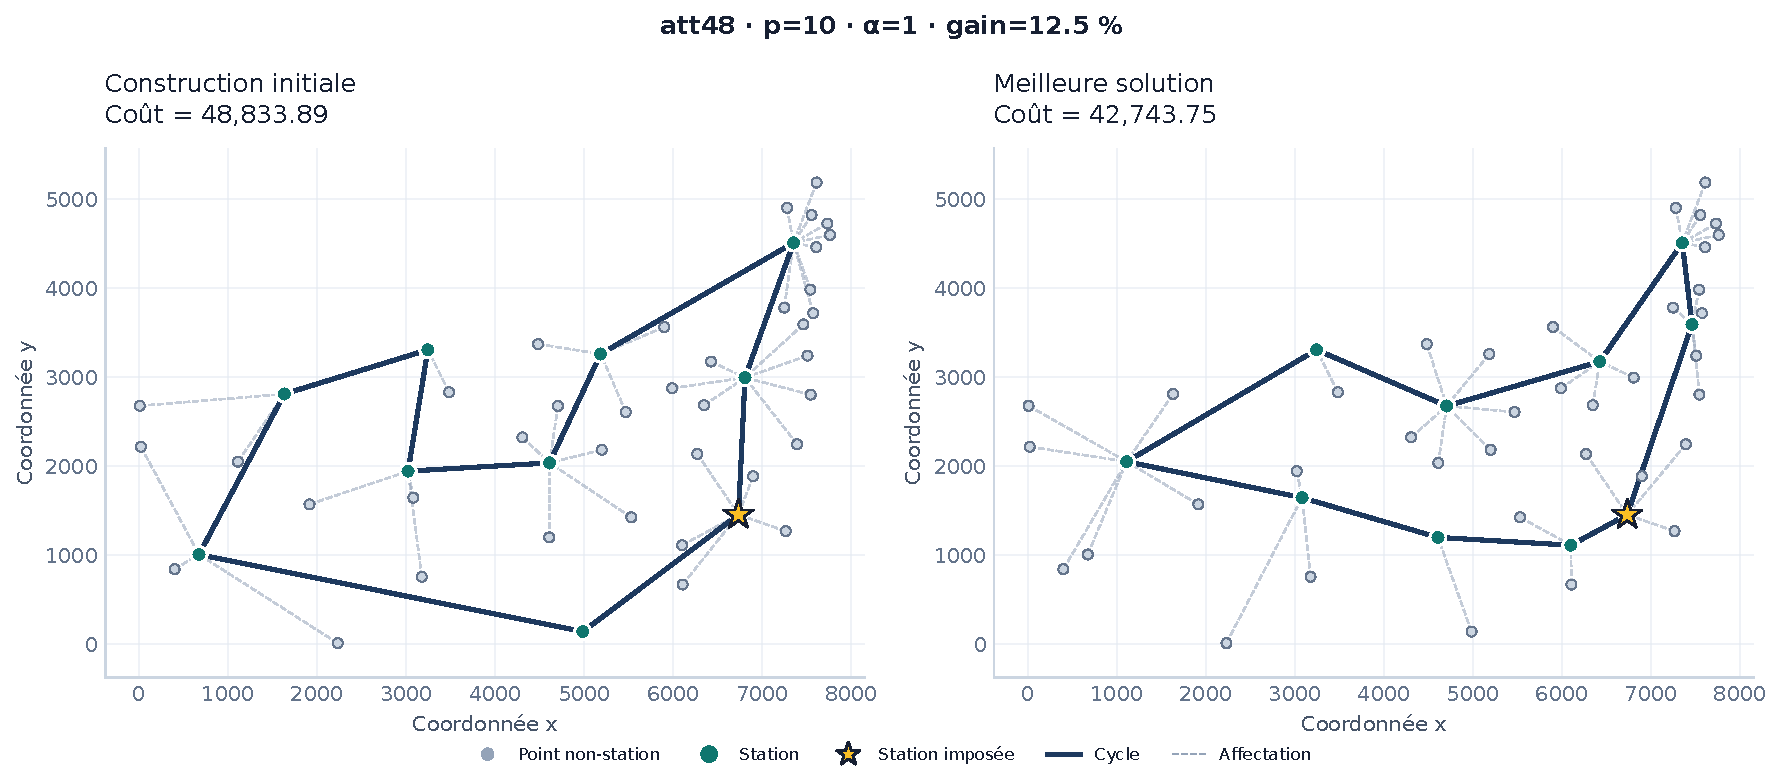
\includegraphics[width=0.99\textwidth]{figures/avant_apres_att48.pdf}
\caption{Att48, dix stations : construction puis meilleure solution tabou
de l'exécution individuelle. L'étoile distingue la station imposée.}
\label{fig:avantapres}
\sourcecalcul{exécution individuelle sauvegardée du 17 octobre 2026,
graine 0 ; 100 itérations, 15 candidats par itération, durée tabou 10.}
\end{figure}

L'anneau est mis en évidence et les traits d'affectation restent plus légers.
Une liaison d'accès plus longue n'est pas nécessairement une erreur : le
problème minimise une somme globale et ne fixe pas de distance maximale
individuelle. Une autre sélection peut donc améliorer le coût total tout en
dégradant l'accès de quelques points.

\section{D'où vient la diminution du coût ?}
Le tableau~\ref{tab:att48-decomp} décompose le résultat. Le coût total passe
de 48\,833,89 à 42\,743,75, soit un gain de 6\,090,14 unités de coordonnées
et une baisse relative de 12,47\,\%. Le README arrondit ce même pourcentage
à 12,5\,\% ; il ne s'agit pas d'un résultat différent.

\begin{table}[htbp]\centering
\begin{tabular}{lrrr}
\toprule
Composante & Construction & Meilleure tabou & Baisse relative \\
\midrule
Longueur de l'anneau & 20\,285{,}26 & 16\,477{,}53 & 18{,}77\,\% \\
Somme des accès & 28\,548{,}63 & 26\,266{,}23 & 7{,}99\,\% \\
Coût total ($\alpha=1$) & 48\,833{,}89 & 42\,743{,}75 & 12{,}47\,\% \\
\bottomrule
\end{tabular}

\caption{Décomposition du coût avant et après la recherche tabou individuelle.}
\label{tab:att48-decomp}
\sourcecalcul{coûts recalculés depuis les solutions initiale et finale sauvegardées.}
\end{table}

Dans cet exemple, les deux composantes diminuent. Ce résultat n'est pas
imposé par la recherche : seul le coût total guide le choix des mouvements.
Sur une autre instance ou avec un autre poids, une amélioration du total
pourrait augmenter l'une des composantes et réduire davantage l'autre.

La meilleure solution sélectionne les stations
$\{1,5,10,13,18,22,30,32,33,34\}$. Son cycle, lu depuis la station imposée,
est
\begin{equation*}
1\to22\to34\to5\to10\to32\to13\to33\to30\to18\to1.
\end{equation*}
L'ordre inverse représente le même cycle non orienté et le même coût.
Les affectations complètes sont conservées dans le fichier JSON de l'exécution,
ce qui permet de vérifier le résultat au-delà de l'image.

\section{Meilleure valeur et solution courante}
La trace de convergence de la figure~\ref{fig:convergence} sépare la meilleure
valeur de la valeur courante. La meilleure solution finale est atteinte
à l'itération 42, après 630 évaluations. La recherche poursuit l'exploration
jusqu'au budget de 100 itérations, sans retrouver de coût plus bas.

Le coût courant à la dernière itération est 45\,535,28, supérieur à la
meilleure valeur 42\,743,75. Ce comportement est attendu dans une recherche
qui accepte des dégradations. Exporter seulement la dernière solution aurait
perdu une partie du gain. Le programme conserve et retourne la meilleure
solution rencontrée, avec l'historique permettant de la situer dans la trajectoire.

\begin{figure}[htbp]\centering
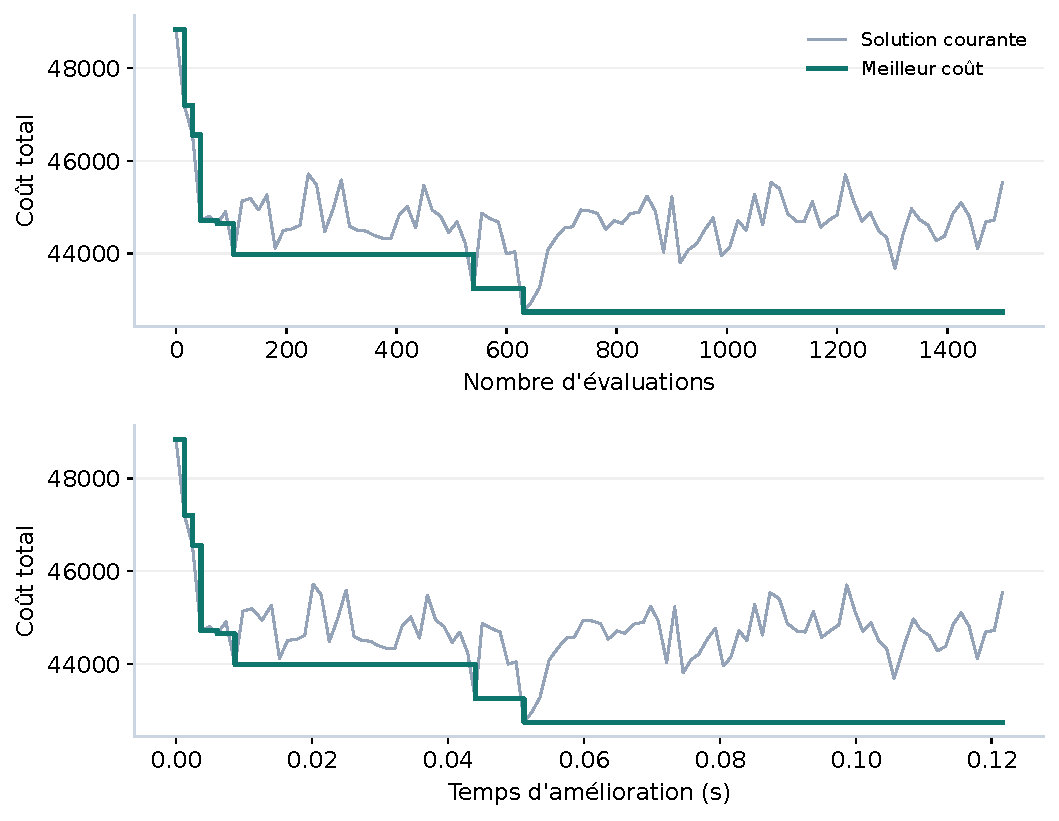
\includegraphics[width=0.98\textwidth]{figures/convergence_att48.pdf}
\caption{Coût courant et meilleure valeur : selon le nombre d'évaluations
en haut, et le temps d'amélioration en bas.}
\label{fig:convergence}
\sourcecalcul{trace sauvegardée dans \code{history.csv} pour l'exécution att48.}
\end{figure}

Le temps d'optimisation complet enregistré est d'environ 0,122 s, tandis que
l'instant d'atteinte du meilleur coût dans la trace est d'environ 0,051 s
après le début de l'amélioration. Ces durées n'incluent pas le dessin des
figures et leurs origines de mesure diffèrent légèrement, comme indiqué
dans le protocole. Leur rôle est d'éclairer cette exécution, sans promettre
la même vitesse sur toute machine.

\section{Portée de cet exemple}
Le gain avant-après est un résultat individuel. La synthèse à trois graines
de la campagne demeure la référence pour comparer les méthodes. L'exemple
ne dispose d'aucune preuve d'optimalité : il montre une amélioration
réalisable, pas la meilleure ligne possible sur les 48 points.

Il illustre aussi une limite du seul coût moyen d'accès. Ni l'accès le plus
long ni les différences entre zones ne sont pénalisés séparément. Pour un
projet de transport réel, une distance d'accès maximale, des poids de
population ou un critère d'équité pourraient modifier sensiblement le tracé.
\bilan{La figure avant-après compare une même instance et une même cardinalité.
La trace explique comment le gain est obtenu et pourquoi la meilleure
solution doit être conservée indépendamment de l'état courant.}

\chapter{Qualité logicielle et limites de l'étude}\label{chap:qualite}
\section{Séparer les responsabilités du programme}
Le noyau représente les instances, les paramètres, les solutions et leurs
règles de validité. Les modules de méthodes construisent ou améliorent des
solutions. Une couche d'exécution commune mesure les calculs et produit un
résultat structuré. Les campagnes orchestrent les cas, tandis que les modules
d'artefacts et de visualisation enregistrent les données et dessinent les figures.

\begin{table}[htbp]\small
\begin{tabularx}{\textwidth}{lL}\toprule
Responsabilité & Modules principaux \\\midrule
Données et modèle & \code{instance}, \code{io}, \code{distances}, \code{solution} \\
Validité & \code{validation} \\
Résolution & \code{heuristics}, \code{metaheuristics}, \code{exact} \\
Exécution et campagnes & \code{execution}, \code{experiments}, \code{benchmark} \\
Résultats et figures & \code{artifacts}, \code{visualization}, \code{experiment_plots} \\
Interface & \code{cli}, point d'entrée \code{ring-star} et Makefile \\
\bottomrule\end{tabularx}
\caption{Organisation des responsabilités dans le projet.}
\end{table}

Cette séparation limite les divergences entre une résolution individuelle
et une campagne : les deux empruntent le même chemin d'exécution. Elle
évite également de reconstruire une solution approximative à partir d'une
simple liste de stations lorsqu'un ordre de cycle sauvegardé existe déjà.

\section{Des résultats autonomes et consultables}
Une exécution sauvegarde les coordonnées, les paramètres, les stations,
le cycle, les affectations, les coûts et les informations de statut.
Les recherches ajoutent la solution initiale et une trace. Le journal CBC
est conservé lorsque cette méthode est utilisée. La campagne fournit un
CSV détaillé, une synthèse statistique et un résumé de complétion.

Les dossiers utilisent un identifiant unique pour éviter les écrasements.
L'index global oriente vers les résolutions individuelles et les campagnes,
puis les résumés guident vers les données et figures pertinentes. Les
figures peuvent être régénérées depuis les solutions sauvegardées sans
disposer du fichier TSPLIB initial et sans relancer l'optimisation.

Les exports PNG facilitent la consultation, tandis que les PDF et SVG
préservent des traits et textes vectoriels pour la rédaction. Les figures
du présent rapport utilisent des PDF du projet, régénérés depuis la synthèse
archivée lorsque nécessaire, sans nouvelle optimisation. Le schéma
de couverture reste l'image fournie par l'auteur, avec son crédit ResearchGate.

\section{Contrôles et tests}
La suite comprend 101 tests. Elle couvre notamment les paramètres invalides,
la lecture des coordonnées, les coûts, les contraintes des solutions,
les méthodes, l'interface, les exports et la disposition des figures.
Des cas limites vérifient les coordonnées dupliquées, un objectif nul,
$p=n$ et les arrêts sans échange possible.

Les contrôles les plus utiles sont ceux qui pourraient détecter un résultat
faux malgré un programme qui s'exécute : comparaison de petites PLNE à une
énumération indépendante, vérification de 2-opt sur l'arête de fermeture,
distinction entre solution entière sous budget et optimum prouvé, rejet
d'un coût sauvegardé incohérent, et relecture des solutions illustrées.
Les campagnes sont testées avec plusieurs poids pour éviter de fusionner
des cas différents dans les synthèses.

Les scripts d'archive et de nettoyage sont aussi testés. Ils doivent préserver
le dépôt Git, l'environnement local et les résultats actuels, et produire
une archive sans dossier enveloppe superflu. Ces vérifications concernent
l'usage du projet autant que ses algorithmes.

Pour la rédaction, les 172 solutions de la campagne ont été relues et leurs
coûts recalculés indépendamment à partir des coordonnées, des cycles et
des affectations. Les moyennes des tableaux ont été rapprochées des coûts
unitaires. Le jeu d'essais de 101 tests a été relancé avec le contrôle
d'export renforcé ; il se termine sans échec dans l'environnement de revue.
Cela ne garantit pas l'absence de tout défaut ni la compatibilité avec
toutes les versions possibles des dépendances.

\section{Un défaut d'export identifié pendant la revue}
Le fichier \code{completion.json} annonce 192 enregistrements et la synthèse
contient les 96 groupes attendus. Le CSV détaillé original n'en contient que
191 : il manque le cas \code{rd100}, $p=10$, PLNE, ignoré par configuration.
Le programme écrivait le CSV après les exécutions calculées, mais pas après
un dernier cas ignoré. Il s'agit donc d'une écriture finale manquante,
sans perte de solution calculée.

Le rapport conserve l'export original et produit une copie réconciliée distincte.
La ligne manquante est reconstituée comme cas ignoré, à partir de la
configuration, de la synthèse et du bilan de complétion. Aucun coût ni
temps de résolution n'est inventé pour ce cas. Les sources incluent le
correctif qui écrit tous les enregistrements à la fin de la campagne,
ainsi qu'une assertion supplémentaire dans le test existant des cas ignorés.
Ce correctif est joint pour intégration au dépôt ; il ne fait pas partie
des trois commits publiés mentionnés au début du rapport.

\section{Limites expérimentales et améliorations prioritaires}
Trois graines donnent un premier aperçu de la variabilité, mais restent peu
nombreuses pour quantifier finement la robustesse des recherches. Les petites
durées sont mesurées une fois par exécution, sans protocole dédié de répétition
ou d'isolation des ressources. La grille constitue une seule référence
constructive : un autre départ pourrait modifier les gains.

La priorité expérimentale serait de comparer les recherches à même nombre
d'évaluations, puis à même budget de temps, avec davantage de graines.
Il serait ensuite utile de faire varier $\alpha$ et $p$ de façon plus large,
d'essayer plusieurs initialisations et de mesurer séparément l'accès,
l'anneau et la distribution des distances individuelles. Une extension de
la PLNE pourrait étudier des relaxations plus fortes ou une formulation
avec séparation de coupes, en mesurant leur apport au-delà du seul temps.

Sur le plan algorithmique, la reconstruction complète de chaque voisin
pourrait être remplacée en partie par des mises à jour incrémentales des
affectations et des modifications locales du cycle. Ce gain de vitesse
demanderait des contrôles supplémentaires pour conserver les mêmes coûts
et ne pas introduire de dépendance cachée à l'état précédent.

Enfin, une application au transport demanderait des distances de réseau,
des demandes, des capacités, des contraintes d'implantation et une prise
en compte de l'équité. Les instances TSPLIB et les unités de coordonnées
ne permettent pas de conclure qu'un tracé proposé serait faisable ou
préférable pour une agglomération réelle.
\bilan{La traçabilité permet de vérifier les résultats et de corriger un
défaut d'export sans modifier les calculs. Les prochaines avancées utiles
portent sur l'équité des budgets, la robustesse des expériences et le
réalisme des données de transport.}

\chapter*{Conclusion générale}
\addcontentsline{toc}{chapter}{Conclusion générale}
Le problème Ring-Star fournit un cadre clair pour étudier ensemble le choix
des stations et leur ordre de desserte sur une ligne circulaire. La
formulation retenue fixe la cardinalité, impose une station et minimise
une somme pondérée de longueur d'anneau et de distances d'accès.
L'intégration du voyageur de commerce comme cas particulier explique sa
NP-difficulté et le besoin de méthodes complémentaires.

La PLNE avec flot exprime directement la sélection, les affectations et
la connexité du cycle. Elle apporte une garantie lorsque CBC termine avec
une preuve, ou une solution réalisable accompagnée d'une borne lorsqu'il
s'arrête avant. Les méthodes approchées ont un rôle différent : construire
rapidement une solution, puis explorer des échanges de stations en
réévaluant les deux composantes de l'objectif.

Sur les 24 cas de la campagne principale, les recherches améliorent les
coûts moyens de la construction. Le gain médian atteint 11,79\,\% pour
la locale et 13,67\,\% pour le tabou. La meilleure moyenne tabou dans
22 cas s'accompagne d'un effort de calcul plus important. Le résultat
doit donc être présenté comme un compromis observé sous des réglages
précis, et non comme une supériorité démontrée à ressources égales.

La comparaison à un optimum est possible sur trois petits cas. Sur
Ulysses16 à cinq stations, les trois trajectoires tabou atteignent le
coût prouvé de 65,3775. Sur les grandes instances, les solutions
restent réalisables et améliorées, sans preuve de leur proximité à
l'optimum. L'exemple att48 illustre cette distinction : une baisse de
12,47\,\% est mesurée par rapport à la construction, avec un coût final
de 42\,743,75, mais sans certificat d'optimalité.

L'organisation des sorties fait partie du résultat du projet. Les
solutions, paramètres, traces et versions permettent de retrouver
l'origine d'un chiffre et de redessiner les figures. La relecture
indépendante des coûts et les tests complètent cette démarche.
Le défaut de dernière ligne ignorée repéré dans le CSV rappelle
l'intérêt de rapprocher les fichiers entre eux, même lorsque les
solutions et les synthèses sont correctes.

La suite du travail peut se concentrer sur des budgets équitables,
davantage de graines et une étude du poids $\alpha$. Une application
opérationnelle demanderait en parallèle de remplacer les distances
planes et les poids uniformes par des données de déplacement,
des demandes et des contraintes réelles. Le projet constitue ainsi
une base expérimentale documentée pour explorer la localisation-routage,
avec des résultats dont la portée et les limites sont explicites.

\chapter*{Glossaire}
\addcontentsline{toc}{chapter}{Glossaire}
\begin{description}
\item[Affectation] Rattachement d'un point à une station ouverte. À stations
fixées et sans capacité, une station la plus proche minimise son coût d'accès.
\item[Anneau] Cycle qui relie toutes les stations sélectionnées et revient
à son point de départ.
\item[Aspiration] Règle qui autorise un mouvement tabou lorsqu'il améliore
la meilleure valeur globale rencontrée.
\item[Borne inférieure] Valeur qui ne dépasse pas l'optimum d'un problème
de minimisation. Sa comparaison à une solution réalisable renseigne
sur l'incertitude d'optimalité.
\item[Campagne] Ensemble d'exécutions décrites par une configuration commune,
avec plusieurs instances, cardinalités, méthodes et éventuellement graines.
\item[Cas expérimental] Problème fixé par l'instance, $p$ et $\alpha$.
Une méthode peut y être exécutée sur plusieurs graines.
\item[CBC] Solveur de programmation entière du projet COIN-OR,
appelé ici à travers PuLP.
\item[Construction] Méthode rapide produisant une première solution réalisable.
Dans le projet : grille, ajustement de cardinalité, affectation, plus proche
voisin et 2-opt.
\item[Écart-type d'échantillon] Mesure descriptive de la dispersion des coûts
entre graines, calculée avec le dénominateur $m-1$.
\item[Évaluation] Reconstruction et calcul du coût d'un voisin candidat.
Une itération peut en contenir plusieurs.
\item[Flot de connexité] Quantité fictive envoyée depuis la racine pour imposer
que toutes les stations appartiennent à une même composante.
\item[Formulation compacte] Modèle dont le nombre de variables et de contraintes
est polynomial en la taille des données ; cette propriété ne rend pas
sa résolution entière nécessairement rapide.
\item[Graine] Valeur qui initialise le générateur pseudo-aléatoire et permet
de reproduire une suite de tirages dans un contexte logiciel donné.
\item[Heuristique] Méthode qui cherche une bonne solution sans garantir
qu'elle soit optimale.
\item[Itération] Étape de la recherche. Dans la campagne, la locale évalue
un voisin par étape et le tabou jusqu'à 15.
\item[Métaheuristique] Stratégie générale d'exploration qui organise les
mouvements, la mémoire et les règles d'acceptation d'une recherche.
\item[NP-difficulté] Propriété qui traduit ici l'inclusion d'un problème
combinatoire difficile comme cas particulier. Elle n'implique pas que
toutes les instances soient difficiles en pratique.
\item[Optimum prouvé] Solution dont le statut du solveur établit l'optimalité,
sous les tolérances numériques utilisées.
\item[PLNE] Programmation linéaire en nombres entiers. Le modèle du rapport
est mixte, car les flots sont continus et les décisions sont binaires.
\item[PuLP] Bibliothèque Python de construction de modèles linéaires et
entiers et d'interface avec des solveurs.
\item[Recherche locale] Exploration d'un voisinage en retenant des améliorations.
La version du projet échantillonne un échange à chaque itération.
\item[Recherche tabou] Recherche avec mémoire temporaire de certains retours,
qui peut accepter une dégradation et conserve la meilleure solution visitée.
\item[Solution réalisable] Solution qui respecte toutes les contraintes,
quelle que soit sa qualité de coût.
\item[TSPLIB] Bibliothèque d'instances de problèmes de tournées. Le projet
en réutilise les coordonnées sous sa propre convention de distance.
\item[Voisinage] Ensemble des solutions accessibles par une règle de mouvement,
ici le retrait d'une station non imposée et l'ajout d'un autre point.
\item[2-opt] Amélioration du cycle par suppression de deux arêtes et inversion
du segment intermédiaire afin de réduire la longueur.
\end{description}

\renewcommand{\bibname}{Références}
\begin{thebibliography}{9}
\addcontentsline{toc}{chapter}{Références}
\bibitem{enonce}
Sup Galilée, Université Sorbonne Paris Nord.
\textit{SAÉ Optimisation 2025-2026 : Autour du tracé d'un métro circulaire}.
Énoncé fourni avec le projet, dix pages ; copie dans
\code{documents/enonce_sae.pdf}. Le périmètre, les hypothèses géométriques
et les objectifs pédagogiques du rapport s'appuient sur ce document.

\bibitem{labbe}
M. Labbé, G. Laporte, I. R. Martín et J. J. Salazar González.
\textit{The Ring Star Problem: Polyhedral Analysis and Exact Algorithm}.
Networks, 43(3), 177-189, 2004. Référence fondatrice indiquée dans
l'énoncé ; le modèle à flot présenté ici décrit l'implémentation du projet,
et non une reproduction revendiquée de l'algorithme de cet article.

\bibitem{figure}
A. Liefooghe, L. Jourdan et E.-G. Talbi.
\textit{Metaheuristics and Their Hybridization to Solve the Bi-objective Ring
Star Problem: a Comparative Study}, 2008.
Illustration « An example of solution for the ring star problem »,
figure diffusée sur
\href{https://www.researchgate.net/figure/An-example-of-solution-for-the-ring-star-problem_fig2_1920886}{researchgate.net}.
Page consultée le 17 octobre 2026. Image de couverture fournie pour le rapport ;
la conversion de WebP en PNG ne modifie ni le tracé ni le cadrage.
Cette référence illustre la structure anneau-étoile, sans constituer une
source des résultats numériques du projet.

\bibitem{tsplib}
G. Reinelt, Université de Heidelberg.
\textit{TSPLIB 95}, page officielle et documentation des instances.
\url{https://comopt.ifi.uni-heidelberg.de/software/TSPLIB95/}.
Consultée le 17 octobre 2026. Les huit fichiers de coordonnées utilisés
sont archivés avec les sources du rapport ; les distances du projet
sont euclidiennes non arrondies, indépendamment du type source.

\bibitem{pulp}
COIN-OR. \textit{PuLP : documentation et constantes de statut}.
\url{https://coin-or.github.io/pulp/technical/constants.html}.
Consultée le 17 octobre 2026. La version utilisée dans les calculs
archivés est PuLP 3.3.2 ; les métadonnées d'exécution font foi pour
cette version, indépendamment de l'évolution du site documentaire.

\bibitem{cbc}
COIN-OR. \textit{Introduction to CBC}.
\url{https://coin-or.github.io/Cbc/intro.html}.
Consultée le 17 octobre 2026. Présentation du solveur de programmation
entière utilisé par le projet.

\bibitem{projet}
\textit{Ring-Star Problem : code, tests et résultats enregistrés}.
Dépôt \href{https://github.com/birane-m/ring-star-problem}{birane-m/ring-star-problem},
état publié au commit \code{8761003}, 17 octobre 2026.
Campagne \code{demo_multi_graines} et exécution individuelle att48 du même jour.
Les données de calcul, l'empreinte des sources expérimentales et les
contrôles de rédaction sont inclus dans \code{resultats/}.
Le correctif d'export joint est identifié séparément.
\end{thebibliography}

\clearpage
\appendix
\renewcommand{\nomChapitre}{ANNEXE}
\chapter{Fichiers, commandes et reproduction}
\section{Installer le projet et vérifier son fonctionnement}
Les commandes suivantes sont à lancer sous Linux depuis la racine du
dépôt. Python 3.10 ou plus récent est déclaré compatible. Les contrôles
décrits dans le rapport ont été exécutés sous Python 3.12. La matrice CI
du dépôt prévoit Python 3.10 et 3.12 ; le rapport ne suppose pas que
l'exécution distante de cette CI a déjà été observée.
\begin{commandes}
git clone https://github.com/birane-m/ring-star-problem.git
cd ring-star-problem
make install
make test
\end{commandes}
Les dépendances sont définies dans \code{pyproject.toml}. Le fichier
\code{requirements.txt} installe le projet en mode éditable et ne
constitue pas une seconde liste indépendante. Les versions de l'exécution
archivée se trouvent dans \code{resultats/campagne/environment.json}.

\section{Reproduire une résolution et une campagne}
L'exemple individuel att48 est paramétré par :
\begin{commandes}
make tabu INSTANCE=data/instances/att48.tsp P=10 ALPHA=1 \
  SEED=0 ITERATIONS=100 CANDIDATES=15 TENURE=10
\end{commandes}
L'interface explicite permet aussi de fixer tous les paramètres :
\begin{commandes}
.venv/bin/ring-star run tabu data/instances/att48.tsp 10 \
  --alpha 1 --seed 0 --iterations 100 \
  --candidates-per-iteration 15 --tabu-tenure 10
\end{commandes}
La campagne de démonstration se lance avec :
\begin{commandes}
make benchmark
\end{commandes}
Elle lit \code{configs/benchmark_demo.json}. Une relance crée un nouveau
dossier horodaté. Les durées, et éventuellement le comportement de CBC
au voisinage du temps limite, peuvent varier. Pour retrouver exactement
les chiffres de ce rapport, utiliser les résultats archivés plutôt que
supposer l'identité des durées d'une nouvelle exécution.

\section{Retrouver les sorties}
\begin{table}[htbp]\small
\begin{tabularx}{\textwidth}{lL}\toprule
Fichier ou dossier & Rôle \\\midrule
\code{outputs/index.md} & Point d'entrée vers les exécutions et campagnes. \\
\code{summary.md} & Lecture d'une résolution, de ses coûts et de ses figures. \\
\code{solution.json} & Coordonnées, solution, paramètres, coûts et statut. \\
\code{initial_solution.json} & Référence initiale d'une recherche. \\
\code{history.csv} & Coûts courant et meilleur, évaluations et temps de recherche. \\
\code{runs.csv} & Enregistrements détaillés des méthodes et graines d'une campagne. \\
\code{summary.csv} & Moyennes, dispersions, statuts et liens aux meilleures graines. \\
\code{completion.json} & État terminé ou interrompu et compte des enregistrements. \\
\code{environment.json} & Versions et empreinte des sources. \\
\code{figures/} & Figures de solution, convergence et comparaison. \\
\bottomrule\end{tabularx}
\caption{Repères de navigation dans les sorties du projet.}
\end{table}
Les anciens chemins absolus présents dans certains fichiers de provenance
documentent leur origine. Les solutions contiennent les coordonnées et
les chemins utiles à la lecture du rapport sont relatifs à ses sources.
La régénération des tableaux ne dépend pas des anciens chemins absolus.

\section{Compiler le rapport et régénérer les tableaux}
L'archive des sources est autonome pour la compilation ; elle contient
les figures utilisées, les tableaux et les résultats qui les alimentent.
Les paquets LaTeX usuels de mathématiques, de langue française et de
mise en page sont nécessaires, ainsi que Python 3 pour les contrôles.
Depuis le dossier contenant \code{main.tex} :
\begin{commandes}
python3 scripts/generer_tableaux.py
latexmk -pdf -interaction=nonstopmode -halt-on-error main.tex
\end{commandes}
Sans \code{latexmk}, compiler \code{main.tex} trois fois avec pdfLaTeX.
La première commande reconstruit les tableaux, vérifie les coûts des
172 solutions et documente le rapprochement des 191 lignes originales
avec les 192 cas attendus. Elle ne lance aucun solveur.

La couverture conserve l'image fournie. Son URL source et ses crédits
sont rassemblés dans \code{IMAGE_SOURCE.txt}. Les figures de résultats
reprennent les exports vectoriels de la campagne et de l'exemple individuel.

\section{Intégrer le correctif d'export au dépôt}
Le fichier \code{correctifs/export_cas_ignores.patch} contient uniquement
l'écriture finale du CSV et le renforcement du test existant. Après avoir
placé les sources du rapport dans \code{reports/latex_ring_star/},
on peut l'appliquer depuis la racine du dépôt :
\begin{commandes}
git apply --check \
  reports/latex_ring_star/correctifs/export_cas_ignores.patch
git apply \
  reports/latex_ring_star/correctifs/export_cas_ignores.patch
make test
\end{commandes}
Le correctif reste à intégrer dans un commit distinct ; l'export original
archivé est conservé.

\chapter{Tableau complet des coûts de la campagne}
Le tableau suivant couvre les 24 problèmes de la campagne, tous avec
$\alpha=1$. La construction est exécutée une fois. Les colonnes locale
et tabou indiquent la moyenne et l'écart-type d'échantillon des trois graines
$0,1,2$. Les valeurs sont exprimées dans les unités de coordonnées de
chaque instance ; elles ne sont pas comparables en valeur brute d'une
instance à l'autre.

Les quatre résolutions PLNE sont présentées séparément au
tableau~\ref{tab:exacts}. Les 20 cas exacts ignorés n'ont aucun coût de
solution à renseigner. Les décimales sont arrondies pour la lecture ;
les JSON conservent la précision de calcul.

\begin{table}[htbp]\centering
{\fontsize{9}{12}\selectfont\setlength{\tabcolsep}{4pt}
\begin{tabular}{lrrrr}
\toprule
Instance & $p$ & Construction & Locale : moyenne $\pm s$ & Tabou : moyenne $\pm s$ \\
\midrule
ulysses16 & 3 & 113{,}31 & 68{,}27 $\pm$ 0{,}00 & 68{,}27 $\pm$ 0{,}00 \\
ulysses16 & 5 & 89{,}19 & 65{,}55 $\pm$ 0{,}15 & 65{,}38 $\pm$ 0{,}00 \\
ulysses16 & 10 & 76{,}44 & 63{,}58 $\pm$ 0{,}39 & 63{,}29 $\pm$ 0{,}02 \\
ulysses22 & 3 & 137{,}72 & 83{,}14 $\pm$ 0{,}00 & 83{,}14 $\pm$ 0{,}00 \\
ulysses22 & 5 & 108{,}79 & 72{,}54 $\pm$ 0{,}83 & 71{,}57 $\pm$ 0{,}00 \\
ulysses22 & 10 & 82{,}36 & 65{,}83 $\pm$ 0{,}25 & 65{,}32 $\pm$ 0{,}07 \\
att48 & 3 & 78\,299{,}77 & 72\,273{,}64 $\pm$ 1\,076{,}65 & 70\,903{,}13 $\pm$ 0{,}00 \\
att48 & 5 & 63\,668{,}04 & 56\,467{,}99 $\pm$ 275{,}98 & 55\,615{,}92 $\pm$ 202{,}51 \\
att48 & 10 & 48\,833{,}89 & 45\,563{,}09 $\pm$ 455{,}55 & 42\,790{,}21 $\pm$ 59{,}20 \\
eil51 & 3 & 859{,}99 & 828{,}26 $\pm$ 0{,}60 & 827{,}57 $\pm$ 0{,}00 \\
eil51 & 5 & 735{,}00 & 708{,}56 $\pm$ 4{,}82 & 698{,}17 $\pm$ 2{,}64 \\
eil51 & 10 & 630{,}47 & 563{,}99 $\pm$ 8{,}93 & 550{,}98 $\pm$ 7{,}44 \\
berlin52 & 3 & 16\,352{,}32 & 14\,095{,}02 $\pm$ 19{,}25 & 14\,090{,}96 $\pm$ 12{,}22 \\
berlin52 & 5 & 14\,916{,}74 & 12\,014{,}92 $\pm$ 148{,}48 & 11\,813{,}49 $\pm$ 22{,}63 \\
berlin52 & 10 & 12\,155{,}57 & 9\,869{,}34 $\pm$ 121{,}56 & 9\,594{,}29 $\pm$ 121{,}71 \\
st70 & 3 & 1\,897{,}37 & 1\,762{,}49 $\pm$ 11{,}55 & 1\,753{,}24 $\pm$ 0{,}00 \\
st70 & 5 & 1\,572{,}53 & 1\,388{,}72 $\pm$ 34{,}01 & 1\,360{,}17 $\pm$ 6{,}86 \\
st70 & 10 & 1\,105{,}82 & 1\,074{,}19 $\pm$ 20{,}63 & 1\,006{,}90 $\pm$ 4{,}32 \\
kroA100 & 3 & 77\,233{,}40 & 76\,618{,}84 $\pm$ 645{,}19 & 75\,202{,}82 $\pm$ 496{,}12 \\
kroA100 & 5 & 68\,427{,}57 & 60\,284{,}12 $\pm$ 1\,653{,}97 & 58\,433{,}18 $\pm$ 59{,}57 \\
kroA100 & 10 & 46\,042{,}25 & 43\,469{,}80 $\pm$ 862{,}27 & 41\,457{,}13 $\pm$ 256{,}17 \\
rd100 & 3 & 30\,724{,}65 & 26\,625{,}74 $\pm$ 394{,}09 & 26\,393{,}33 $\pm$ 17{,}48 \\
rd100 & 5 & 21\,243{,}25 & 20\,528{,}93 $\pm$ 567{,}28 & 19\,541{,}48 $\pm$ 55{,}80 \\
rd100 & 10 & 16\,692{,}42 & 14\,072{,}26 $\pm$ 254{,}50 & 13\,604{,}29 $\pm$ 163{,}40 \\
\bottomrule
\end{tabular}
}
\caption{Coûts moyens de construction, recherche locale et recherche tabou,
sur tous les cas de la campagne de démonstration.}
\sourcetable
\end{table}
\FloatBarrier

La source détaillée originale est \code{resultats/campagne/runs.csv}.
La copie \code{resultats/runs_reconcilies.csv} ajoute uniquement le cas
PLNE ignoré terminal, sans solution ni coût. Le fichier
\code{resultats/provenance_rapport.json} décrit cette opération et conserve
les empreintes des fichiers ayant servi à la rédaction.

\chapter{Notations et conventions de lecture}
\begin{table}[htbp]\small
\begin{tabularx}{\textwidth}{lL}\toprule
Symbole & Définition \\\midrule
$V$, $n$ & Ensemble des points et nombre de points. \\
$r$ & Station imposée, usuellement le premier sommet. \\
$p$, $S$ & Nombre de stations et ensemble sélectionné, avec $|S|=p$. \\
$d_{ij}$ & Distance euclidienne non arrondie dans le plan des coordonnées. \\
$\pi$ & Permutation des stations ; le retour à la première est implicite. \\
$a(i)$ & Station affectée au point $i$. \\
$L$, $A$ & Longueur du cycle et somme des distances d'accès. \\
$\alpha$, $C$ & Poids du cycle et coût total $C=\alpha L+A$. \\
$z_i$, $y_{ij}$ & Variables binaires de station et d'affectation. \\
$x_{ij}$, $f_{ij}$ & Variable binaire d'arête et flot continu de connexité. \\
$B$, $C^*$ & Borne inférieure et optimum prouvé lorsqu'il est disponible. \\
$\overline C$, $s_C$ & Moyenne et écart-type d'échantillon des coûts par graine. \\
$G$ & Gain relatif face à la construction du même cas. \\
$g^*$ & Écart de coût à un optimum prouvé, en pourcentage. \\
$g_B$ & Écart entre une solution et la borne du solveur, rapporté à $|C|$. \\
\bottomrule\end{tabularx}
\caption{Notations principales utilisées dans le rapport.}
\end{table}

\section{Indices et cycle fermé}
Le rapport et les listes exportées utilisent la numérotation à partir de 1.
Les structures Python utilisent des indices à partir de 0. Les coordonnées
de \code{problem} dans un JSON sont dans l'ordre interne ; les listes de
stations, de cycle et d'affectations lisibles sont numérotées à partir de 1.
Le champ interne \code{problem.required_station} ne doit donc pas être
comparé directement à une liste exportée sans conversion.

Le cycle est enregistré sous forme d'une permutation de longueur $p$.
La station initiale n'est pas répétée en dernière position dans cette liste.
Le calcul de longueur ajoute toujours l'arête de fermeture. Le cycle
$1,2,3$ désigne ainsi $1\to2\to3\to1$.

\section{Statuts d'exécution}
\code{ok} désigne une exécution heuristique réussie ; il ne signifie pas
optimal. \code{optimal} indique une preuve issue du solveur.
\code{feasible_time_limited} signale une solution réalisable sans preuve
dans le budget. \code{skipped} correspond à un cas volontairement non lancé.
Les erreurs ou absences de solution ont des statuts distincts et ne doivent
pas être transformées en coûts nuls pour calculer une moyenne.

\end{document}
